\section{LabVIEW als Programmiersprache}
	\label{sec:labview}
	
LabVIEW ist ein grafisches Programmiersystem von National Instruments. Das Akronym steht für "`Laboratory Virtual Instrumentation Engineering Workbench"'.

Die Programmierung erfolgt in der graphischen Programmiersprache "`G"'.  LabVIEW-Programme werden als Virtuelle Instrumente (VIs) bezeichnet. \cite{ni-tuto}
%\cite{wiki-lv}

Sie bestehen aus drei Komponenten: 
\begin{description}
	\item[Frontpanel] Das User-Interface, über welches der Anwender mit dem VI interagiert.
	\item[Blockdiagramm] Stellt den Programmcode des VIs dar.
	\item[Anschluss] Dient zur Anbindung an weitere VIs. Bestimmt Übergabe und Rückgabe Werte. 
\end{description}

In LabVIEW liegt die Ausführung von VIs dem Datenflussmodell zugrunde. Ein Blockdiagrammknoten (Bsp. Addition) wird ausgeführt, sobald all seine Eingänge belegt sind. Ist die Ausführung eines Knotens abgeschlossen, werden die Daten an die Ausgabeanschlüsse übergeben und die Ausgabedaten dann an den nächsten Knoten im Datenflussdiagramm weitergeleitet. \cite{LVT}
Die unter LabVIEW erstellten Blockdiagramme werden von einem grafischen Compiler in optimierten Maschinencode übersetzt. Dadurch ist die Performance vergleichbar mit der anderer Hochsprachen wie C oder Pascal. \cite{ni-compiler}

Abbildung \ref{fig:demo01} zeigt eine kleine Demonstration. Es wird aus den Eingängen A und B ein Ausgang C berechnet. Die Formel wird im Blockdiagramm abgebildet. Sie lautet:
\[ C = \frac{A+B}{4}^{2} \]
Des Weiteren findet die Berechnung in einer While-Schleife statt. Die Abbruchbedingung ist die Betätigung der Stopp-Schaltfläche. 

	\begin{figure}%[h!]
	\centering
		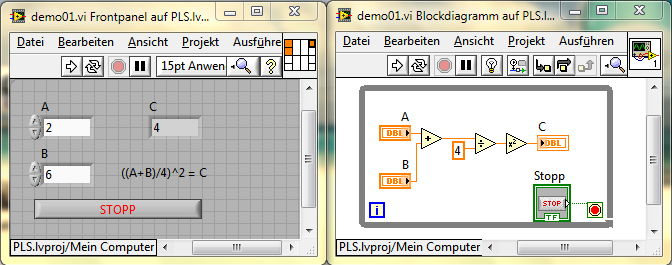
\includegraphics[width=0.7\textwidth]{Pics/demo01.png}
	\caption{VI Demonstration: Links Frontpanel, Rechts Blockdiagramm}
	\label{fig:demo01}
	\end{figure}

	%\subsection{Objektorientiertes Design}  %2-15
	\subsection{Entwurfsmuster - Design Pattern}
		\subsubsection{Master/Slave}
		\subsubsection{Zustandsautomat}%4-6
		\subsubsection{Erzeuger Verbraucher Design} %4-10 Erzeuger / Verbraucher / 
		\paragraph{Event Handling}
		\paragraph{Error Handling} %4-47
		
\section{Programm Analyse}
		\subsection{Programmablaufplan} %2-18
		\subsection{Ablaufdiagramm }
		\subsection{Datenfluss Diagramm}
		
\section{User Interface}

\section{Code Implementierung}
		\subsection{Auswahl des Design Pattern} %6-3
		\subsection{Timing}
		\subsection{Auswahl der Datentypen}

		\subsection{Init und Shutdown Funktion}	%E 7-1
		\subsection{Aufnahme-Funktion}	
		\subsection{Abspiel-Funktion}
		\subsection{Stopp-Funktion}
		\subsection{Speichern und Lade Funktion}
			
		\subsection{Fehlerbehandlung}

\section{Testen}		

\section{Anwendung}
	\subsection{Stand-Alone Applikation}
	\subsection{Installer}
	\subsection{Webservice}

\section{Abschließende Betrachtung}
	\subsection{Update }%E8-2
	\subsection{Information Hidding} %E4-5
	\subsection{Erweiterungen}
	Hardware Ansteuerung, Visualisierung größer

